%%%%%%%%%%%%%%%%%%%%%%%%%%%%%%%%%%%%%%%%%%%
%%%%%%%%%%%%%%%%%%%%%%%%%%%%%%%%%%%%%%%%%%%
%%%%%%%%%%%%%%% CHAPTER 04 %%%%%%%%%%%%%%%%


\section{Equações diferenciais ordinárias}

\frame{
\frametitle{Definições}
\begin{block}{Equação diferencial}
Uma equação cuja incógnita é uma função e onde aparece alguma derivada desta função é uma equação diferencial (\textbf{ED}).
\end{block}
}

\frame{
\frametitle{Definições}
\begin{block}{Equação diferencial ordinária}
\begin{itemize}
    \item Se a função incógnita é de uma variável, a ED é ordinária (\textbf{EDO}), pois nela só aparecem as derivadas "comuns"\ (derivadas ordinárias).
    \item Se a função incógnita é de várias variáveis, a ED é parcial (\textbf{EDP}), pois como a função tem mais de uma variável, aparecem derivadas parciais.
\end{itemize}
\end{block}
}

\frame{
\frametitle{Definições}
\begin{block}{Ordem de uma EDO}
\begin{itemize}
    \item Chama-se \textbf{ordem} de uma EDO a "maior"\ derivada que aparece na equação.
    \item Exemplo $\#01$: $x \dfrac{\text{d}^2y}{\text{d}x^2} - \dfrac{\text{d}y}{\text{d}x} = 2$ é de ordem dois (ou de segunda ordem).
    \item Exemplo $\#02$: $x\text{d}y - y\text{d}x = 0$ é de ordem um (ou de primeira ordem).
\end{itemize}
\end{block}
}

\frame{
\frametitle{Definições}
\begin{block}{EDO homogênea}
\begin{itemize}
    \item Uma EDO é \textbf{homogênea} quando não há termo independente nem da função incógnita nem de sua(s) derivadas(s).
    \item Exemplo $\#01$: $x\text{d}y - e^y \text{d}x = 0$ é homogênea.
    \item Exemplo $\#02$: $x^2 + x^\prime = \text{cos}(t)$ não é homogênea.
\end{itemize}
\end{block}
}

\frame{
\frametitle{Definições}
\begin{block}{EDO linear}
\begin{itemize}
    \item Uma EDO é \textbf{linear} quando pode ser escrita como uma espécie de "polinômio"\ $a_0y + a_1y^\prime + a_2y^{\prime\prime} + \cdots + a_ny^{(n)} =g(x)$, onde a função incógnita é $y(x)$, os coeficientes $a_0, a_1, a_2, \cdots, a_n$ são constantes ou funções de $x$, e $g(x)$ é uma função qualquer.
    \item Observe que nem a função nem suas derivadas aparecem como argumentos de funções trigonométricas, exponenciais, logarítmicas, etc.
    \item Exemplo $\#01$: $y^{\prime\prime} + t^2y = e^t$ é linear.
    \item Exemplo $\#02$: $ \dfrac{\text{d}^2y}{\text{d}x^2} + \dfrac{\text{d}y}{\text{d}x} + \text{cos}(y)= 0$ não é linear ($\text{cos}(y)$).
    \item Exemplo $\#03$: $ \dfrac{\text{d}x}{\text{d}t} - 2t^2x + 2\text{cos}(t)\dfrac{\text{d}^2x}{\text{d}t^2}= 0$ é linear.
    \item Exemplo $\#04$: $x^2 + x^\prime = \text{cos}(t)$ não é linear ($x^2$).
\end{itemize}
\end{block}
}

\frame{
\frametitle{Definições - Exemplo $\#01$}
\begin{block}{Pêndulo}
O movimento de um pêndulo simples de massa $m$ e comprimento $L$ é descrito pela função $\theta(t)$ -- função incógnita -- que satisfaz a EDO
\vspace{-0.2cm}
$$\dfrac{\text{d}^2 \theta}{\text{d}t^2} + \dfrac{g}{L} \text{sen}(\theta) = 0$$
\vspace{-0.4cm}
\begin{itemize}
    \item $\theta$ é a \textbf{variável dependente} e $t$ é a \textbf{variável independente}.
\end{itemize}
\end{block}
\centerline{
\includegraphics[width=0.37\linewidth]{Figuras/Ch04/fig1.png}}
}

\frame{
\frametitle{Definições - Exemplo $\#02$}
\begin{block}{Circuito RC série}
Um circuito $RC$ é aquele que tem um resistor de resistência $R$, um capacitor de capacitância $C$, além de um gerador que cria uma diferença de potencial $V(t)$, ligados em série. A carga $Q(t)$ no capacitor -- função incógnita -- satisfaz a EDO
\vspace{-0.2cm}
$$R\dfrac{\text{d}Q}{\text{d}t} + \dfrac{1}{C} Q = V(t)$$
\vspace{-0.4cm}
\begin{itemize}
    \item $Q$ é a \textbf{variável dependente} e $t$ é a \textbf{variável independente}.
\end{itemize}
\end{block}
\centerline{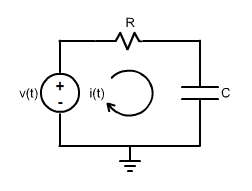
\includegraphics[width=0.4\linewidth]{Figuras/Ch04/fig3.PNG}}
}

\frame{
\frametitle{Solução de uma EDO}
\begin{block}{Definição}
\begin{itemize}
    \item Resolver uma EDO significa determinar \textbf{todas as funções} que a satisfazem. Tais funções formam uma \textbf{família de soluções} da EDO (solução geral).
    \item O número de constantes que aparecem na expressão algébrica da família de soluções é igual à ordem da EDO.
    \item Para resolver uma EDO não homogênea devemos:
        \begin{enumerate}
            \item Obter uma solução $y_h(t)$ da \textbf{equação homogênea}.
            \item Obter uma solução particular $y_p(t)$ da \textbf{equação não homogênea}.
            \item A \textbf{solução geral} da EDO é $\boxed{y(t) = y_h(t) + y_p(t)}$.
        \end{enumerate}
\end{itemize}
\end{block}
}

\frame{
\frametitle{Problema de valor inicial}
\begin{block}{Definição}
\begin{itemize}
    \item Uma condição que deve ser satisfeita pela solução $y$ de uma EDO em um valor $t_0$ é chamada de \textbf{condição inicial}. Uma EDO com uma condição inicial é chamada de \textbf{problema de valor inicial (PVI)}.
\end{itemize}
\end{block}
}

\frame{
\frametitle{Exemplo $\#01$ - EDO não homogênea}
\begin{block}{Problema}
Resolver a EDO abaixo:
$$y^{\prime\prime} - 2y^{\prime} - 3y = e^t$$
\end{block}
}

\frame{
\frametitle{Exemplo $\#01$ - EDO não homogênea}
\begin{block}{Resolução - método tradicional}
\begin{itemize}
    \item O primeiro passo é encontrar a solução homogênea $y_h(t)$: \\
\end{itemize}
\vspace{0.2cm}
$y^2 - 2y - 3 = 0$ possui raízes em $y = -1$ e $y = 3$. Deste modo,
$$y_h(t) = C_1 e^{-t} + C_2 e^{3t}$$
\end{block}
}

\frame{
\frametitle{Exemplo $\#01$ - EDO não homogênea}
\begin{block}{Resolução - método tradicional}
\begin{itemize}
    \item O segundo passo é encontrar a solução particular $y_p(t)$: \\
\end{itemize}
\vspace{0.2cm}
Uma "candidata"\ a $y_p(t)$ é $g(t) = e^{t}$. Logo, 
$$y_p(t) = Ae^{t} \ \therefore \ y_p^{\prime} = y_p^{\prime\prime} = Ae^{t}$$
Substituindo na EDO original, temos:
$$Ae^{t} - 2Ae^{t} -3 Ae^{t} = e^{t} \implies A = -\dfrac{1}{4}$$
Com isso,
$$y_p(t) = -\dfrac{1}{4} e^{t}$$
\end{block}
}

\frame{
\frametitle{Exemplo $\#01$ - EDO não homogênea}
\begin{block}{Resolução - método tradicional}
\begin{itemize}
    \item A solução geral da EDO é $y(t) = y_h(t) + y_p(t)$:
\end{itemize}
$$\boxed{y(t) = -\dfrac{1}{4} e^{t} + C_1 e^{-t} + C_2 e^{3t}}$$
\end{block}
}

\frame{
\frametitle{Exemplo $\#01$ - EDO não homogênea}
\begin{block}{Resolução - transformada de Laplace}
\begin{itemize}
    \item A transformada de Laplace também pode ser usada para resolver equações diferenciais ordinárias, não apenas PVIs. Lembre-se apenas que a equação diferencial ordinária tem que ser linear, de coeficientes constantes, e a transformada de Laplace da parte não homogênea tem que existir. Ao invés de valores numéricos para $y(0)$ e $y^{\prime}(0)$, teremos constantes, por exemplo: $y(0) = K$ e $y^{\prime}(0) = P$.
\end{itemize}
$$s^2 Y(s) - sy(0) - y^{\prime}(0) - 2\big(s Y(s) - y(0)\big) - 3 Y(s) = \frac{1}{s-1}$$
$$s^2 Y(s) - Ks -P - 2s Y(s) + 2K - 3 Y(s) = \frac{1}{s-1}$$
$$Y(s) = \frac{1}{(s-1)(s^2-2s-3)} + \frac{Ks + P - 2K}{s^2-2s-3}$$
\end{block}
}

\frame{
\frametitle{Exemplo $\#01$ - EDO não homogênea}
\begin{block}{Resolução - transformada de Laplace}
\begin{itemize}
    \item Invertendo o primeiro termo de $Y(s)$ temos:
\end{itemize}
$$\frac{1}{(s-1)(s+1)(s-3)} = \frac{A}{s-1} + \frac{B}{s+1} + \frac{C}{s-3}$$
$$A = F(s)(s-1)\Big|_{s=1} = \dfrac{1}{(s+1)(s-3)}\Big|_{s=1} = -1/4$$
$$B = F(s)(s+1)\Big|_{s=-1} = \dfrac{1}{(s-1)(s-3)}\Big|_{s=-1} = 1/8$$
$$C = F(s)(s-3)\Big|_{s=3} = \dfrac{1}{(s-1)(s+1)}\Big|_{s=3} = 1/8$$
\vspace{-0.3cm}
\begin{itemize}
    \item Deste modo, a transformada inversa de Laplace da primeira parte é dada por:
\end{itemize}
$$\mathscr{L}^{-1}\ \Big\{-\dfrac{1/4}{s-1} + \dfrac{1/8}{s+1} + \dfrac{1/8}{s-3}\ \Big\}= -\frac{1}{4}e^{t} + \frac{1}{8}e^{-t}+\frac{1}{8}e^{3t}$$
\end{block}
}

\frame{
\frametitle{Exemplo $\#01$ - EDO não homogênea}
\begin{block}{Resolução - transformada de Laplace}
\begin{itemize}
    \item Invertendo o segundo termo de $Y(s)$ temos:
\end{itemize}
$$\frac{Ks + P - 2K}{(s+1)(s-3)} = \frac{D}{s+1} + \frac{E}{s-3}$$
$$D = F(s)(s+1)\Big|_{s=-1} = \dfrac{Ks + P - 2K}{s-3}\Big|_{s=-1} = (3K - P)/4$$
$$E = F(s)(s-3)\Big|_{s=3} = \dfrac{Ks + P - 2K}{s+1}\Big|_{s=3} = (K+P)/4$$
\vspace{-0.3cm}
\begin{itemize}
    \item Deste modo, a transformada inversa de Laplace da segunda parte é dada por:
\end{itemize}
$$\mathscr{L}^{-1}\ \Big\{\dfrac{(3K - P)/4}{s+1} + \dfrac{(K+P)/4}{s-3}\ \Big\}= \frac{3K - P}{4}e^{-t}+\frac{K + P}{4}e^{3t}$$
\end{block}
}

\frame{
\frametitle{Exemplo $\#01$ - EDO não homogênea}
\begin{block}{Resolução - transformada de Laplace}
\begin{itemize}
    \item Aplicando a propriedade da superposição, obtemos:
\end{itemize}
$$y(t) = -\frac{1}{4}e^{t} + \frac{1}{8}e^{-t}+\frac{1}{8}e^{3t} + \frac{3K - P}{4}e^{-t}+\frac{K + P}{4}e^{3t}$$
$$y(t) = -\frac{1}{4}e^{t} + \Big(\frac{1}{8} + \frac{3K - P}{4}\Big) e^{-t} + \Big(\frac{1}{8} + \frac{K + P}{4}\Big) e^{3t}$$
$$\boxed{y(t) = -\dfrac{1}{4} e^{t} + C_1 e^{-t} + C_2 e^{3t}}$$
\end{block}
}

\frame{
\frametitle{Exemplo $\#02$ - EDO homogênea}
\begin{block}{Problema}
Resolver a EDO abaixo:
$$y^{\prime\prime} - 2y^{\prime} - 3y = 0$$
\end{block}
}

\frame{
\frametitle{Exemplo $\#02$ - EDO homogênea}
\begin{block}{Resolução - método tradicional}
\begin{itemize}
    \item O primeiro passo é encontrar a solução homogênea $y_h(t)$: \\
\end{itemize}
\vspace{0.2cm}
$y^2 - 2y - 3 = 0$ possui raízes em $y = -1$ e $y = 3$. Deste modo,
$$y_h(t) = C_1 e^{-t} + C_2 e^{3t}$$
\end{block}
}

\frame{
\frametitle{Exemplo $\#02$ - EDO homogênea}
\begin{block}{Resolução - método tradicional}
\begin{itemize}
    \item Como essa EDO é homogênea, temos que $y_p(t) = 0$
\end{itemize}
\begin{itemize}
    \item A solução geral da EDO é $y(t) = y_h(t) + y_p(t)$:
\end{itemize}
$$\boxed{y(t) = C_1 e^{-t} + C_2 e^{3t}}$$
\end{block}
}

\frame{
\frametitle{Exemplo $\#02$ - EDO homogênea}
\begin{block}{Resolução - transformada de Laplace}
\begin{itemize}
    \item A transformada de Laplace também pode ser usada para resolver equações diferenciais ordinárias, não apenas PVIs. Lembre-se apenas que a equação diferencial ordinária tem que ser linear, de coeficientes constantes, e a transformada de Laplace da parte não homogênea tem que existir. Ao invés de valores numéricos para $y(0)$ e $y^{\prime}(0)$, teremos constantes, por exemplo: $y(0) = K$ e $y^{\prime}(0) = P$.
\end{itemize}
$$s^2 Y(s) - sy(0) - y^{\prime}(0) - 2\big(s Y(s) - y(0)\big) - 3 Y(s) = 0$$
$$s^2 Y(s) - Ks -P - 2s Y(s) + 2K - 3 Y(s) = 0$$
$$Y(s) = \frac{Ks + P - 2K}{s^2-2s-3}$$
\end{block}
}

\frame{
\frametitle{Exemplo $\#02$ - EDO homogênea}
\begin{block}{Resolução - transformada de Laplace}
\begin{itemize}
    \item Invertendo $Y(s)$ temos:
\end{itemize}
$$\frac{Ks + P - 2K}{(s+1)(s-3)} = \frac{A}{s+1} + \frac{B}{s-3}$$
$$A = F(s)(s+1)\Big|_{s=-1} = \dfrac{Ks + P - 2K}{s-3}\Big|_{s=-1} = (3K - P)/4$$
$$B = F(s)(s-3)\Big|_{s=3} = \dfrac{Ks + P - 2K}{s+1}\Big|_{s=3} = (K+P)/4$$
\vspace{-0.3cm}
\begin{itemize}
    \item Deste modo, a transformada inversa de Laplace é dada por:
\end{itemize}
$$\mathscr{L}^{-1}\ \Big\{\dfrac{(3K - P)/4}{s+1} + \dfrac{(K+P)/4}{s-3}\ \Big\}= \frac{3K - P}{4}e^{-t}+\frac{K + P}{4}e^{3t}$$
\end{block}
}

\frame{
\frametitle{Exemplo $\#02$ - EDO homogênea}
\begin{block}{Resolução - transformada de Laplace}
\begin{itemize}
    \item Logo,
\end{itemize}
$$y(t) = \frac{3K - P}{4}e^{-t}+\frac{K + P}{4}e^{3t}$$
$$\boxed{y(t) = C_1 e^{-t} + C_2 e^{3t}}$$
\end{block}
}

\frame{
\frametitle{Exemplo $\#03$ - EDO não homogênea com PVI}
\begin{block}{Problema}
Resolver o PVI abaixo:
$$y^{\prime\prime} - y = -2te^{-t} \qquad y(0) = 1, \ y^{\prime}(0) = -1$$
\end{block}
}

\frame{
\frametitle{Exemplo $\#03$ - EDO não homogênea com PVI}
\begin{block}{Resolução - método tradicional}
\begin{itemize}
    \item O primeiro passo é encontrar a solução homogênea $y_h(t)$: \\
\end{itemize}
\vspace{0.2cm}
$y^2 - 1 = 0$ possui raízes em $y = 1$ e $y = -1$. Deste modo,
$$y_h(t) = C_1 e^{t} + C_2 e^{-t}$$
\end{block}
}

\frame{
\frametitle{Exemplo $\#03$ - EDO não homogênea com PVI}
\begin{block}{Resolução - método tradicional}
\begin{itemize}
    \item O segundo passo é encontrar a solução particular $y_p(t)$: \\
\end{itemize}
\vspace{0.2cm}
Uma "candidata"\ a $y_p(t)$ é $g(t) = (At^2+Bt)e^{-t}$. Logo,
$$y_p^{\prime} = (-At^2 + (2A - B)t + B)e^{-t}$$
$$y_p^{\prime\prime} = (At^2 + (-4A + B)t + 2A-2B)e^{-t}$$
Substituindo na EDO original, temos:
$$(-4At - 2B + 2A)e^{-t} = -2te^{-t} \implies A = \dfrac{1}{2}, B = \dfrac{1}{2}$$
Com isso, 
$$y_p(t) = \dfrac{1}{2}t^2e^{-t} + \dfrac{1}{2}te^{-t}$$
\end{block}
}

\frame{
\frametitle{Exemplo $\#03$ - EDO não homogênea com PVI}
\begin{block}{Resolução - método tradicional}
\begin{itemize}
     \item A solução geral da EDO é $y(t) = y_h(t) + y_p(t)$:
\end{itemize}
$$y(t) = C_1 e^{t} + C_2 e^{-t} + \dfrac{1}{2}t^2e^{-t} + \dfrac{1}{2}te^{-t}$$
\end{block}
}

\frame{
\frametitle{Exemplo $\#03$ - EDO não homogênea com PVI}
\begin{block}{Resolução - método tradicional}
\begin{itemize}
    \item Aplicando o PVI, obtemos:
\end{itemize}
$$y(0) = 1 \implies C_1 + C_2 = 1$$
$$y^{\prime}(0) = -1 \implies C_1 - C_2 = -\dfrac{3}{2}$$
Resolvendo este sistema de equações encontramos $C_1 = -\dfrac{1}{4}$ e $C_2 = \dfrac{5}{4}$
\begin{itemize}
    \item Logo, a solução geral do PVI é:
\end{itemize}
$$\boxed{y(t) = -\dfrac{1}{4}e^{t} + \dfrac{5}{4}e^{-t} + \dfrac{1}{2}t^2e^{-t} + \dfrac{1}{2}te^{-t}}$$
\end{block}
}

\frame{
\frametitle{Exemplo $\#03$ - EDO não homogênea com PVI}
\begin{block}{Resolução - transformada de Laplace}
\begin{itemize}
    \item "Laplaceando"\ ambos os membros, e usando as propriedades, vem:
\end{itemize}
$$s^2 Y(s) - sy(0) - y^{\prime}(0) - Y(s) = -2 \dfrac{1}{(s+1)^2}$$
$$s^2 Y(s) - s -(-1) - Y(s) = -2 \dfrac{1}{(s+1)^2}$$
$$Y(s)(s^2 - 1) =  s -1 + \dfrac{-2}{(s+1)^2}$$
$$Y(s) = \dfrac{1}{s+1} + \dfrac{-2}{(s+1)^3(s-1)}$$
\begin{itemize}
    \item A transformada inversa de Laplace do primeiro termo é dada diretamente, via tabela, como $e^{-t}$
\end{itemize}
\end{block}
}

\frame{
\frametitle{Exemplo $\#03$ - EDO não homogênea com PVI}
\begin{block}{Resolução - transformada de Laplace}
\begin{itemize}
    \item Invertendo o segundo termo, temos:
\end{itemize}
$$\frac{-2}{(s+1)^3(s-1)} = \frac{A}{s+1} + \frac{B}{(s+1)^2} + \frac{C}{(s+1)^3} + \frac{D}{s-1}$$
$$\frac{-2}{(s+1)^3(s-1)} = \frac{A}{s+1} + \frac{B}{(s+1)^2} + \frac{2C}{(s+1)^3} + \frac{D}{s-1}$$
$$-2 = A(s+1)^2(s-1) + B(s+1)(s-1) + 2C(s-1) + D(s+1)^3$$
Resolvendo o sistema, temos $A = \dfrac{1}{4}$, $B = \dfrac{1}{2}$, $C = \dfrac{1}{2}$ e $D = -\dfrac{1}{4}$
\begin{itemize}
    \item Deste modo, a transformada inversa de Laplace da segunda parte é dada por:
\end{itemize}
$$\mathscr{L}^{-1}\ \Big\{\dfrac{1/4}{s+1} + \dfrac{1/2}{(s+1)^2} + \dfrac{1/2 \cdot 2}{(s+1)^3} - \dfrac{1/4}{s-1}\ \Big\} = \dfrac{1}{4} e^{-t} + \dfrac{1}{2} te^{-t} + \dfrac{1}{2} t^2e^{-t} - \dfrac{1}{4} e^{t}$$
\end{block}
}

\frame{
\frametitle{Exemplo $\#03$ - EDO não homogênea com PVI}
\begin{block}{Resolução - transformada de Laplace}
\begin{itemize}
    \item Logo, a solução geral do PVI é:
\end{itemize}
$$\boxed{y(t) = -\dfrac{1}{4}e^{t} + \dfrac{5}{4}e^{-t} + \dfrac{1}{2}t^2e^{-t} + \dfrac{1}{2}te^{-t}}$$
\end{block}
}

\frame{
\frametitle{Exemplo $\#04$ - EDO homogênea com PVI}
\begin{block}{Problema}
Resolver o PVI abaixo:
$$y^{\prime\prime} - 2y^{\prime} -3y = 0 \qquad y(0) = -1, \ y^{\prime}(0) = 2$$
\end{block}
}

\frame{
\frametitle{Exemplo $\#04$ - EDO homogênea com PVI}
\begin{block}{Resolução - método tradicional}
\begin{itemize}
    \item O primeiro passo é encontrar a solução homogênea $y_h(t)$: \\
\end{itemize}
\vspace{0.2cm}
$y^2 - 2y -3 = 0$ possui raízes em $y = -1$ e $y = 3$. Deste modo,
$$y_h(t) = C_1 e^{-t} + C_2 e^{3t}$$
\end{block}
}

\frame{
\frametitle{Exemplo $\#04$ - EDO homogênea com PVI}
\begin{block}{Resolução - método tradicional}
\begin{itemize}
    \item Como essa EDO é homogênea, temos que $y_p(t) = 0$
\end{itemize}
\begin{itemize}
    \item A solução geral da EDO é $y(t) = y_h(t) + y_p(t)$:
\end{itemize}
$$y(t) = C_1 e^{-t} + C_2 e^{3t}$$
\end{block}
}

\frame{
\frametitle{Exemplo $\#04$ - EDO homogênea com PVI}
\begin{block}{Resolução - método tradicional}
\begin{itemize}
    \item Aplicando o PVI, obtemos:
\end{itemize}
$$y(0) = -1 \implies C_1 + C_2 = -1$$
$$y^{\prime}(0) = 2 \implies -C_1 +3C_2 = 2$$
Resolvendo este sistema de equações encontramos $C_1 = -\dfrac{5}{4}$ e $C_2 = \dfrac{1}{4}$
\begin{itemize}
    \item Logo, a solução geral do PVI é:
\end{itemize}
$$\boxed{y(t) = -\dfrac{5}{4}e^{-t} + \dfrac{1}{4}e^{3t}}$$
\end{block}
}

\frame{
\frametitle{Exemplo $\#04$ - EDO homogênea com PVI}
\begin{block}{Resolução - transformada de Laplace}
\begin{itemize}
    \item "Laplaceando"\ ambos os membros, e usando as propriedades, vem:
\end{itemize}
$$s^2 Y(s) - sy(0) - y^{\prime}(0) - 2\big(sY(s) - y(0)\big) -3 Y(s) = 0$$
$$s^2 Y(s) + s -2 - 2sY(s) -2 -3Y(s) = 0$$
$$Y(s)(s^2-2s-3) = -s+4$$
$$Y(s) = \dfrac{-s+4}{s^2-2s-3}$$
\end{block}
}

\frame{
\frametitle{Exemplo $\#04$ - EDO homogênea com PVI}
\begin{block}{Resolução - transformada de Laplace}
\begin{itemize}
    \item Invertendo $Y(s)$, temos:
\end{itemize}
$$\frac{-s+4}{(s+1)(s-3)} = \frac{A}{s+1} + \frac{B}{s-3}$$
$$A = F(s)(s+1)\Big|_{s=-1} = \dfrac{-s+4}{s-3}\Big|_{s=-1} = -5/4$$
$$B = F(s)(s-3)\Big|_{s=3} = \dfrac{-s+4}{s+1}\Big|_{s=3} = 1/4$$
\begin{itemize}
    \item Deste modo, a transformada inversa de Laplace é dada por:
\end{itemize}
$$\mathscr{L}^{-1}\ \Big\{-\dfrac{5/4}{s+1} + \dfrac{1/4}{s-3}\ \Big\} = -\dfrac{5}{4} e^{-t} + \dfrac{1}{4} e^{3t}$$
\end{block}
}

\frame{
\frametitle{Exemplo $\#04$ - EDO homogênea com PVI}
\begin{block}{Resolução - transformada de Laplace}
\begin{itemize}
    \item Logo, a solução geral do PVI é:
\end{itemize}
$$\boxed{y(t) = -\dfrac{5}{4} e^{-t} + \dfrac{1}{4} e^{3t}}$$
\end{block}
}

\frame{
\frametitle{Exercícios}
\begin{block}{}
01. Encontre a solução do PVI $y^{\prime\prime} - 3y^{\prime} +2y = 4e^{2t}; \quad y(0) = -3, y^{\prime}(0) = 5$

\vspace{0.5cm}

02. A equação diferencial para a carga em um capacitor em um circuito em série RC é
$$R \dot{q}(t) + \dfrac{1}{C}q(t) = E(t),$$
onde $R$ é a resistência, $C$ é a capacitância e $E(t)$ é a força eletromotriz (f.e.m.).
Determinar, usando as transformadas de Laplace, a carga do capacitor em um circuito RC série se $q(0) = 0$, $R = \SI{2,5}{\ohm}$, $C = \SI{0,08}{\farad}$ e $E(t)$ é dado pelo gráfico abaixo.
\end{block}
\centerline{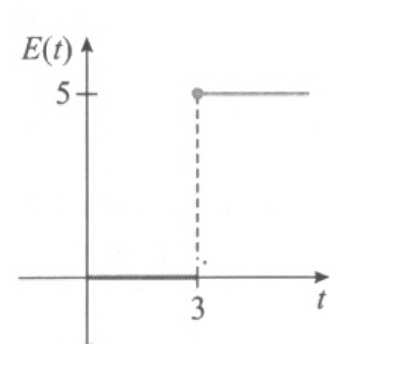
\includegraphics[width=0.27\linewidth]{Figuras/Ch04/fig2.PNG}}
}

\frame{
\frametitle{Referências e exercícios complementares}
\begin{itemize}
\item LATHI, Bhagwandas P. Sinais e Sistemas Lineares, 2 ed. Bookman, 2007.
\end{itemize}
\centering{\alert{Página 214 - \textbf{Capítulo 2}}} \\
}



